\documentclass{article}
\usepackage[ruled,vlined,linesnumbered,resetcount]{algorithm2e}
\usepackage[bottom=8em]{geometry}
\usepackage{amsmath, amssymb, amsthm, enumerate, hyperref}
\usepackage{color}
\usepackage{setspace}
\usepackage{fancyhdr,lastpage}
\usepackage{url}
\usepackage{tabularx}
\usepackage{tikz}
\pagestyle{fancy}
\lhead{\footnotesize Problem Set 3}
\chead{}
\rhead{\footnotesize CS 4150 - Fall 2020}
\lfoot{}
\cfoot{\small \thepage/\pageref*{LastPage}}
\rfoot{}


\newcommand{\pname}[1]{\textnormal{\textsc{#1}}}

\newtheorem*{theorem}{Theorem}
\newtheorem{definition}{Definition}
\newtheorem*{lemma}{Lemma}

\begin{document}

{\it Please enter your name and uID below.}

\vspace{3em}

\makebox[4.3cm]{Name: Qianlang Chen}
\par
\makebox[4.3cm]{uID: u1172983}
\par

\vfill

\subsubsection*{Submission notes}
\begin{itemize}
  \item Due at 11:59 pm on Friday, October 23.
  \item Solutions must be typeset using one of the template files. For each problem, your answer must fit
    in the space provided (e.g. not spill onto the next page) *without* space-saving tricks
    like font/margin/line spacing changes.
  \item Upload a PDF version of your completed problem set to Gradescope.
  \item Teaching staff reserve the right to request original source/tex files during the grading process, so please retain these until an assignment has been returned.
  \item Please remember that for problem sets, collaboration with other students must be limited to a high-level discussion of solution strategies. If you do collaborate with other students in this way, you must identify the students and describe the nature of the collaboration. You are not allowed to create a group solution, and all work that you hand in must be written in your own words. Do not base your solution on any other written solution, regardless of the source.
\end{itemize}

\pagebreak


\begin{enumerate}

  \item (Choosing Candy)

    Let $x_1$ and $x_2$ respectively represent the number of bags of Good \& Plenty and Necco Wafers the professor should buy. Now, we can build a linear program (in canonical form) for this problem:
    $$
      \begin{aligned}
         & \text{maximize}      & -5x_1 - 3x_2              \\
         & \text{subjective to} & -45x_1 - 30x_2 & \le -450 \\
         &                      & x_1            & \le 10   \\
         &                      & x_2            & \le 8    \\
         &                      & -x_1 + x_2     & \le 0    \\
         &                      & x_1, x_2       & \ge 0
      \end{aligned}
    $$
    This plot shows the feasible region for this linear program (in green shadow) and the line representing ``spending 60 dollars'' (in red):
    \begin{center}
      \href{https://www.desmos.com/calculator/amudvktrfc}{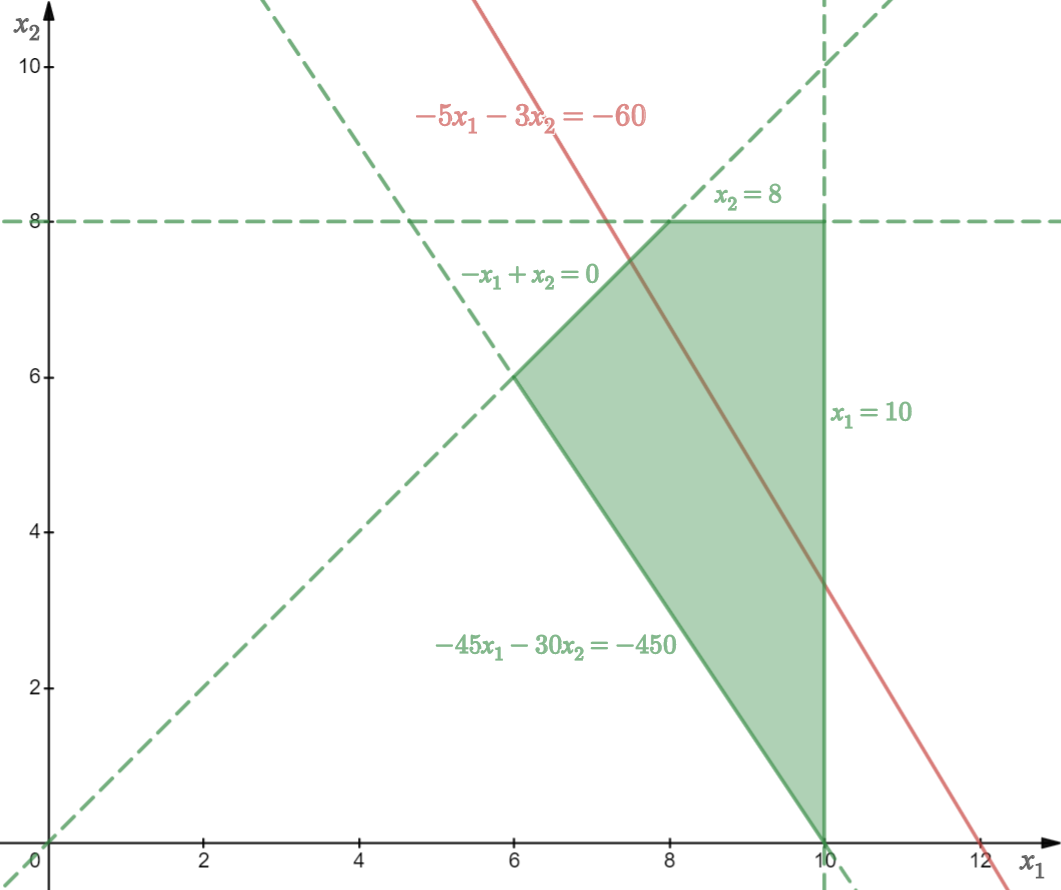
\includegraphics[width=0.75\linewidth]{images/q1b_1.png}}
    \end{center}
    Since the optimal solution in this case must occur on one of the corners of the feasible region, let's calculate the objective function value at each corner:
    $$
      \begin{array}{|cc|c|}
        \hline
        x_1 & x_2 & \text{Objective function value} \\
        \hline
        10  & 0   & -5 \times 10 - 3 \times 0 = -50 \\
        \hline
        10  & 8   & -5 \times 10 - 3 \times 8 = -74 \\
        \hline
        8   & 8   & -5 \times 8 - 3 \times 8 = -64  \\
        \hline
        6   & 6   & -5 \times 6 - 3 \times 6 = -48  \\
        \hline
      \end{array}
    $$
    Since we turned the objective function into a maximizing function by taking the opposite of the expression, the output values are all opposite as well. The table tells us that $-48$ is the optimal solution to the above linear program, and the corresponding spending is 48 dollars for the professor, which is done by buying 6 bags of Necco Wafers and 6 bags of Good \& Plenty.

    \pagebreak

  \item (LP Duality)

    It turned out that the optimal solution occurred at buying 6 bags of each, which is located at the lower left corner of the plot. Removing the shelf-constraints would only extend the region forever to the top and to the right, and since this is a linear program, any point in the extended region cannot possibly do better than this optimal solution located at lower-left, meaning that the current optimal solution would still be an optimal solution in the new linear program.

    After removing the shelf-constraints, let's create the dual of the original linear program, which should have same optimal solution:
    $$
      \begin{aligned}
         & \text{minimize}      & -450y_1                \\
         & \text{subjective to} & -45y_1 - y_2  & \ge -5 \\
         &                      & -30y_1  + y_2 & \ge -3 \\
         &                      & y_1, y_2      & \ge 0
      \end{aligned}
    $$
    The feasible region of the above linear program is as follows:
    \begin{center}
      \href{https://www.desmos.com/calculator/8gugxk2gyv}{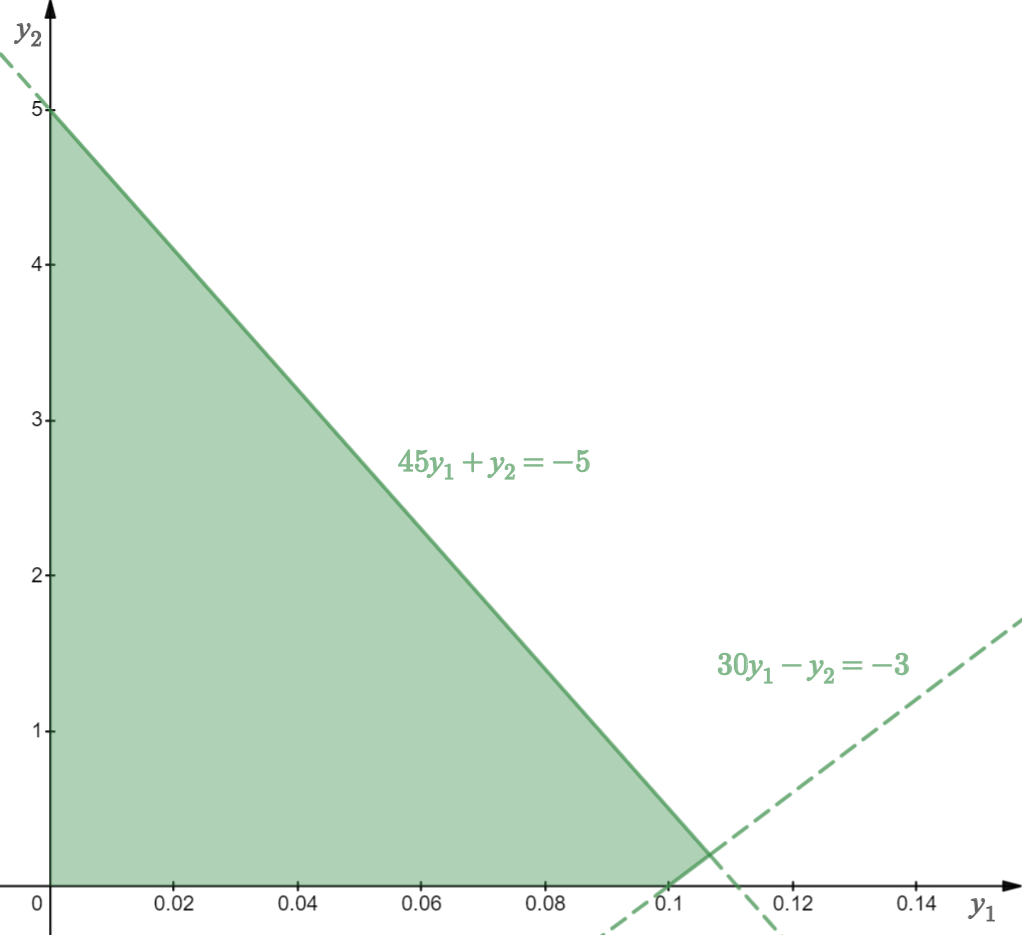
\includegraphics[width=0.6667\linewidth]{images/q2c_1.png}}
    \end{center}
    Again, since the feasible region is bounded, the optimal solution must occur at one of its corners:
    $$
      \begin{array}{|cc|c|}
        \hline
        y_1           & y_2          & \text{Objective function value} \\
        \hline
        0             & 0            & -450 \times 0 = 0               \\
        \hline        &              &                                 \\[-10pt]
        \dfrac{1}{10} & 0            & -450 \times \dfrac{1}{10} = -45 \\[6pt]
        \hline        &              &                                 \\[-10pt]
        \dfrac{8}{75} & \dfrac{1}{5} & -450 \times \dfrac{8}{75} = -48 \\[6pt]
        \hline
        0             & 5            & -450 \times 0 = 0               \\
        \hline
      \end{array}
    $$
    As seen from the table, the optimal solution of this linear program is also $-48$.

    \pagebreak

  \item (Complement Connectivity)

    \textbf{Proof.} Let some disconnected graph $G = (V, E)$ be given. Let the complement of $G$ be called $\bar{G} = (V, [V^2] \setminus E)$, and let $\bar{E} = [V^2] \setminus E$. Note that $V$ must have at least two vertices because otherwise $G$ wouldn't be disconnected anymore. So, let any two vertices $u, v \in V$ be given. One of the following cases about $u$ and $v$ must be true:
    \begin{itemize}
      \item \textbf{Case 1,} $u$ and $v$ are in the same connected component in $G$. Since $G$ is disconnected, $G$ must have some other connected component different from the one containing $u$ and $v$. Let some vertex $w$ from the other component be given. Since $w$ is in a different component than both $u$ and $v$, we know that $uw \notin E$ and $vw \notin E$, meaning that $uw, vw \in \bar{E}$, implying that there's a walk from $u$ to $v$ in $\bar{G}$ and that $u$ and $v$ are in the same component in $\bar{G}$.
      \item \textbf{Case 2,} $u$ and $v$ are not in the same connected component in $G$, so we know that $uv \notin E$. This immediately implies that $uv \in \bar{E}$, which means that there's a walk from $u$ to $v$ in $\bar{G}$ and that $u$ and $v$ are in the same component in $\bar{G}$.
    \end{itemize}
    Now, we've shown that $u$ and $v$ are always in the same connected component in $\bar{G}$. Since $\bar{G}$ and $G$ share the same vertex set, $\bar{G}$ can only have one connected component and is therefore connected. $\square$

    \pagebreak

  \item (Greedy Coloring, Part 1)

    \textbf{(a) Proof.} Let's assume that the algorithm \texttt{GreedyColoring} uses more than $\Delta + 1$ colors for some graph $G$, where $\Delta$ is the highest degree in $G$. Now, let's see why this cannot happen.

    Apart from the initialization of the array \texttt{color} at line 4, the algorithm sets the color for each vertex $i$ at line 9, where $i$ gets the color equal to the minimum value in the set $V$. We know that $V$ was defined to be $S \setminus C$, where $C$ is the set of colors that $i$'s neighbors have and $S$ is the constant set $\{1, 2, \cdots, n\}$. If the algorithm uses more than $\Delta + 1$ colors, there must be some vertex $i$ that's got assigned a color more than $\Delta + 1$ since 1 is the smallest color the algorithm uses (1 is the smallest element in $S$). By the assignment process we've just described, it means that the minimum value in $S \setminus C$ is greater than $\Delta + 1$, which can only happen when $C \supseteq \{1, 2, \cdots, \Delta + 1\}$. In other words, $i$ has neighbors who are colored $\{1, 2, \cdots, \Delta + 1\}$, but this would mean that $i$ has at least $\Delta + 1$ neighbors, which would disagree with the fact that $\Delta$ was the highest degree in $G$. Such vertex $i$ cannot exist, and such graph $G$ cannot exist, so our assumption in the beginning must've been wrong. The algorithm \texttt{GreedyColoring} always uses at most $\Delta + 1$ colors for any graph. $\square$

    \textbf{(b)} After all, when assigning a color for a vertex $i$, we're only interested in the minimum value in $S \setminus C$, which is the smallest color that hasn't appeared within $i$'s neighbors. Since such smallest color can only be at most (deg($i$) + 1), we can use an array of this size to mark the appeared colors and loop again at the end to find the smallest unmarked color:
    \begin{center}
      \begin{minipage}{0.5625\linewidth}
        \renewcommand{\thealgocf}{}
        \SetArgSty{textrm}
        \begin{algorithm}[H]
          \caption{\texttt{GreedyColoring}}
          \KwIn{\tt set<int> A[1..n]}
          \KwOut{\tt int[1..n]}

          {\tt int color[1..n]} $\gets$ filled with 0

          \setcounter{AlgoLine}{5}

          \For{{\tt int i} from 1 to {\tt n}}
          {
            {\tt int deg} $\gets$ length of {\tt A[i]}

              {\tt bool mark[1..deg]} $\gets$ filled with {\tt false}

            \For{each {\tt \textbf{int} nei} in {\tt A[i]}}
            {
              \If{1 $\le$ {\tt color[nei]} $\le$ {\tt deg}}
              {
                {\tt mark[color[nei]]} $\gets$ {\tt true}
              }
            }

            {\tt int min} $\gets$ 1

            \While{{\tt min} $\le$ {\tt deg} and {\tt mark[min]}}
            {
              {\tt min} $\gets$ {\tt min} + 1
            }

            {\tt color[i]} $\gets$ {\tt min}
          }

          \Return{{\tt color}}
        \end{algorithm}
      \end{minipage}
    \end{center}

    \textbf{(c)} First of all, it's easy to see that the initialization of the array \texttt{color} (lines 3-5 from the original pseudocode) takes $O(V)$ time. Now, the main for-loop (lines 6-10) iterates exactly $V$ times, and each iteration takes an additional $O$(deg($i$)) for vertex $i$; in total, the main for-loop takes $O(V) + O$(deg(1)) + $O$(deg(2)) + $\cdots$ + $O$(deg($V$)). Since we know for a fact that the degrees of any (undirected) graph sum to twice the number of edges, the main for-loop will take $O(V + 2 \cdot E) = O(V + E)$ time. Therefore, the entire algorithm takes $O(V + E)$.

    \pagebreak

  \item (Greedy Coloring, Part 2)

    \textbf{(a)} Let's introduce the following strategy for building a bipartite graph $G_n$ with an even number of vertices $n \ge 2$:
    \begin{itemize}
      \item Create $n$ vertices named $1, 2, \cdots, n$.
      \item For each odd vertex $j$ from 3 up to $n - 1$, create edges that connect $j$ to all even vertices up to $j - 1$. (For example, connect vertex 7 to vertices 2, 4, and 6.)
      \item For each even vertex $k$ from 4 up to $n$, create edges that connect $k$ to all odd vertices up to $k - 3$. (For example, connect vertex 8 to vertices 1, 3, and 5.)
    \end{itemize}
    It's easy to see that this strategy will create a bipartite graph, with the even and odd numbers being the two partite sets, since we only create edges between vertices with different parities.

    Now, let's see why a graph $G_n = (V_n, E_n)$ created by this strategy makes \texttt{GreedyColoring} use $n/2$ colors:
    \begin{itemize}
      \item \textbf{Claim.} For any even number $k$ where $2 \le k \le n$, the algorithm \texttt{GreedyColoring} uses the colors $1..(k/2)$ for all odd vertices up to $k-1$ and for all even vertices up to $k$.
      \item \textbf{Proof.} Let's induct on $k$:

        \underline{Base case:} Since the algorithm colors in vertices in numerical order, the vertices 1 and 2 will both get the color 1 because there isn't an edge between vertices 1 and 2. This shows that the claim holds for $k = 2$.

        \underline{Inductive Step:} Assume that the claim holds for some $k = i$ (even), meaning that all odd vertices up to $i-1$ have $i/2$ different colors and similarly for all even vertices up to $i$. The algorithm will have to give the vertex $i+1$ the color $(i/2) + 1 = (i+2)/2$ because the vertex $i+1$ is connected to all the even vertices up to $i$ that already have the colors $1..(i/2)$. Similarly, the vertex $i+2$ will also get the color $(i+2)/2$ because it's connected to all the odd vertices up to $i-1$ that already have the colors $1..(i/2)$. This shows that the claim holds for $k = i+2$, which completes the inductive step and shows that the claim is true for $k = n$. $\square$
    \end{itemize}
    Since we know that a bipartite graph can be colored using at most two colors, the graph $G_n$ shows that the algorithm \texttt{GreedyColoring} doesn't always produce the optimal coloring.

    \textbf{(b)} Here's an example graph $G$:
    $$G = (V, E); V = \{1, 2, 3\}, E = \{\{1, 2\}, \{1, 3\}, \{2, 3\}\}$$

    \textbf{(c)} No, there are permutations on such graphs where \texttt{PermutedGreedy} doesn't produce a suboptimal coloring. (That is, there are situations where \texttt{PermutedGreedy} will produce an optimal coloring.) Imagine a bipartite graph created with the strategy from \textit{part (a)} that has at least four vertices. Consider a permutation that lists all odd vertices before the even ones. Since there are no edges between any two vertices from the same partite set, the algorithm will give all the odd vertices the color 1 and then give all the even vertices the color 2 since 1 is the only color appeared within the neighbors of any even vertex. Only two colors are used given this permutation, which is optimal.

\end{enumerate}

\end{document}
